\begin{enumerate}
    \item Se estudia la aproximación a un filtro pasa bajos mediante al truncamiento de la respuesta a impulso haciendo uso  de una ventana rectangular  con el filtro dado por 
    
 $$   
h[n]= \left\{ \begin{array}{lcc}
             \frac{w_c}{pi}~sinc(\frac{w_c}~{\pi} (n- \frac{N-1}{2})) &   ,  & n = 0,1,..., N-1 \\
             \\ 0 &  ,  & e.o.c \\
  
             \end{array}
   \right.  
   $$


Donde $\omegaw_c$ corresponde a la frecuencia de corte del filtro, en este caso este parámetro tomará el valor de $\frac{2\pi}{3}$

Se crean tres filtros con $N = 21,~ 101,~ 1001$, para los cuales se obtuvieron las siguientes gráficas para la magnitud  y fase de su respuesta en frecuencia utilizando la función \texttt{DTFT.mat}.

\begin{figure}[H]
    \centering
    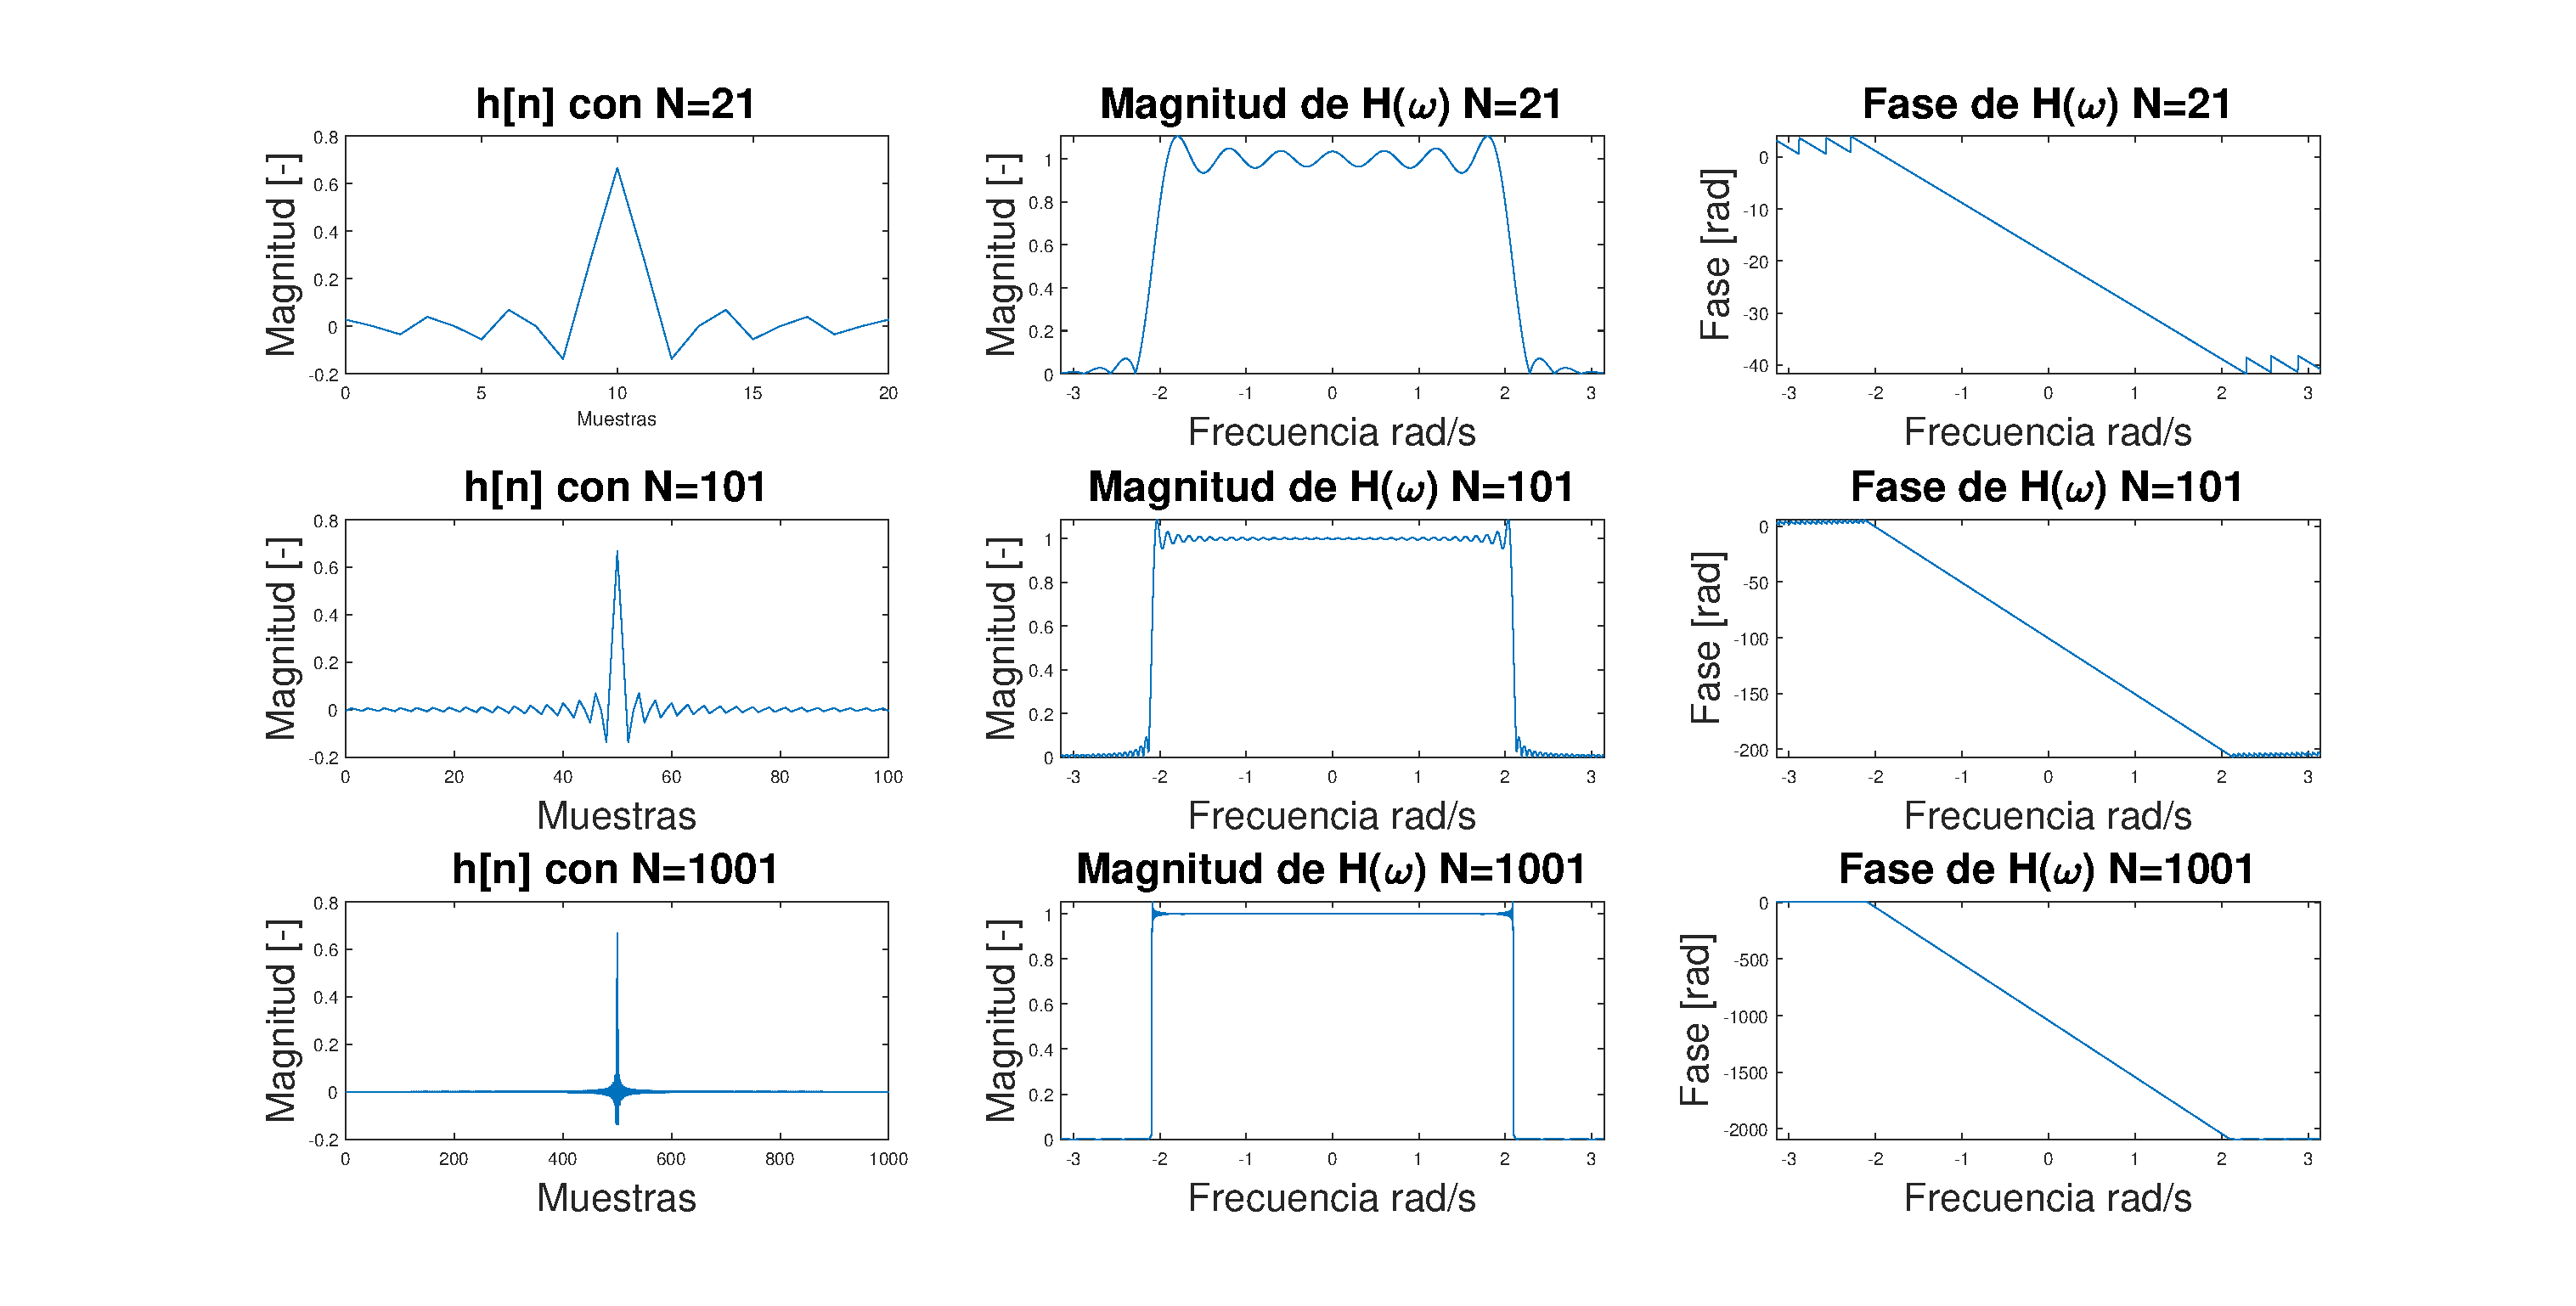
\includegraphics[scale = 0.3]{Figuras/p2_1-Sincs.eps}
    \caption{Magnitud y fase de la respuesta en frecuencia para los filtros de ventana rectangular con  con $N = 21,~ 101,~ 1001$}
    \label{}
\end{figure}

Se puede observar que, como era de esperarse, una ventana con un valor de N mayor genera una respuesta en frecuencia más prolija, con menos ripple y con pendientes más pronunciadas en las frecuencias de corte acercándose de esta forma a el comportamiento de un filtro ideal, al utilizar un valor de N menor la respuesta en frecuencia se puede distorsionar debido a la presencia clara de ripple y la atenuación de las frecuencias posteriores a la frecuencia de corte no es tan efectiva.

Lo mismo ocurre con la fase, mientras más elevado es el valor de N para el filtro, la respuesta en la fase se vuelve más plana en las frecuencias que superan en magnitud a la frecuencia de corte del filtro, mientras que las frecuencias que no se atenúan por el filtro para todos los valores de N evaluados se comportan de forma similar.



\item Para comparar las propiedades espectrales y temporales de los filtros FIR construidos se hace uso de las ventanas predefinidas por MATLAB:  \texttt{freqz}, \texttt{rectwin}, \texttt{hann}, \texttt{hamming},
\texttt{blackman}, y \texttt{bartlett}; que corresponden a las ventanas de tipo   rectangular, hamming, hanning, blackman, y bartlett respectivamente.  Esto utilizando $1 ~kps$ como tasa de muestreo de cada ventana y una duración de $100~ms$.

En la figura \ref{ventanas_tiempo} se puede observar el comportamiento en el tiempo para cada tipo de ventana.

\begin{figure}[H]
    \centering
    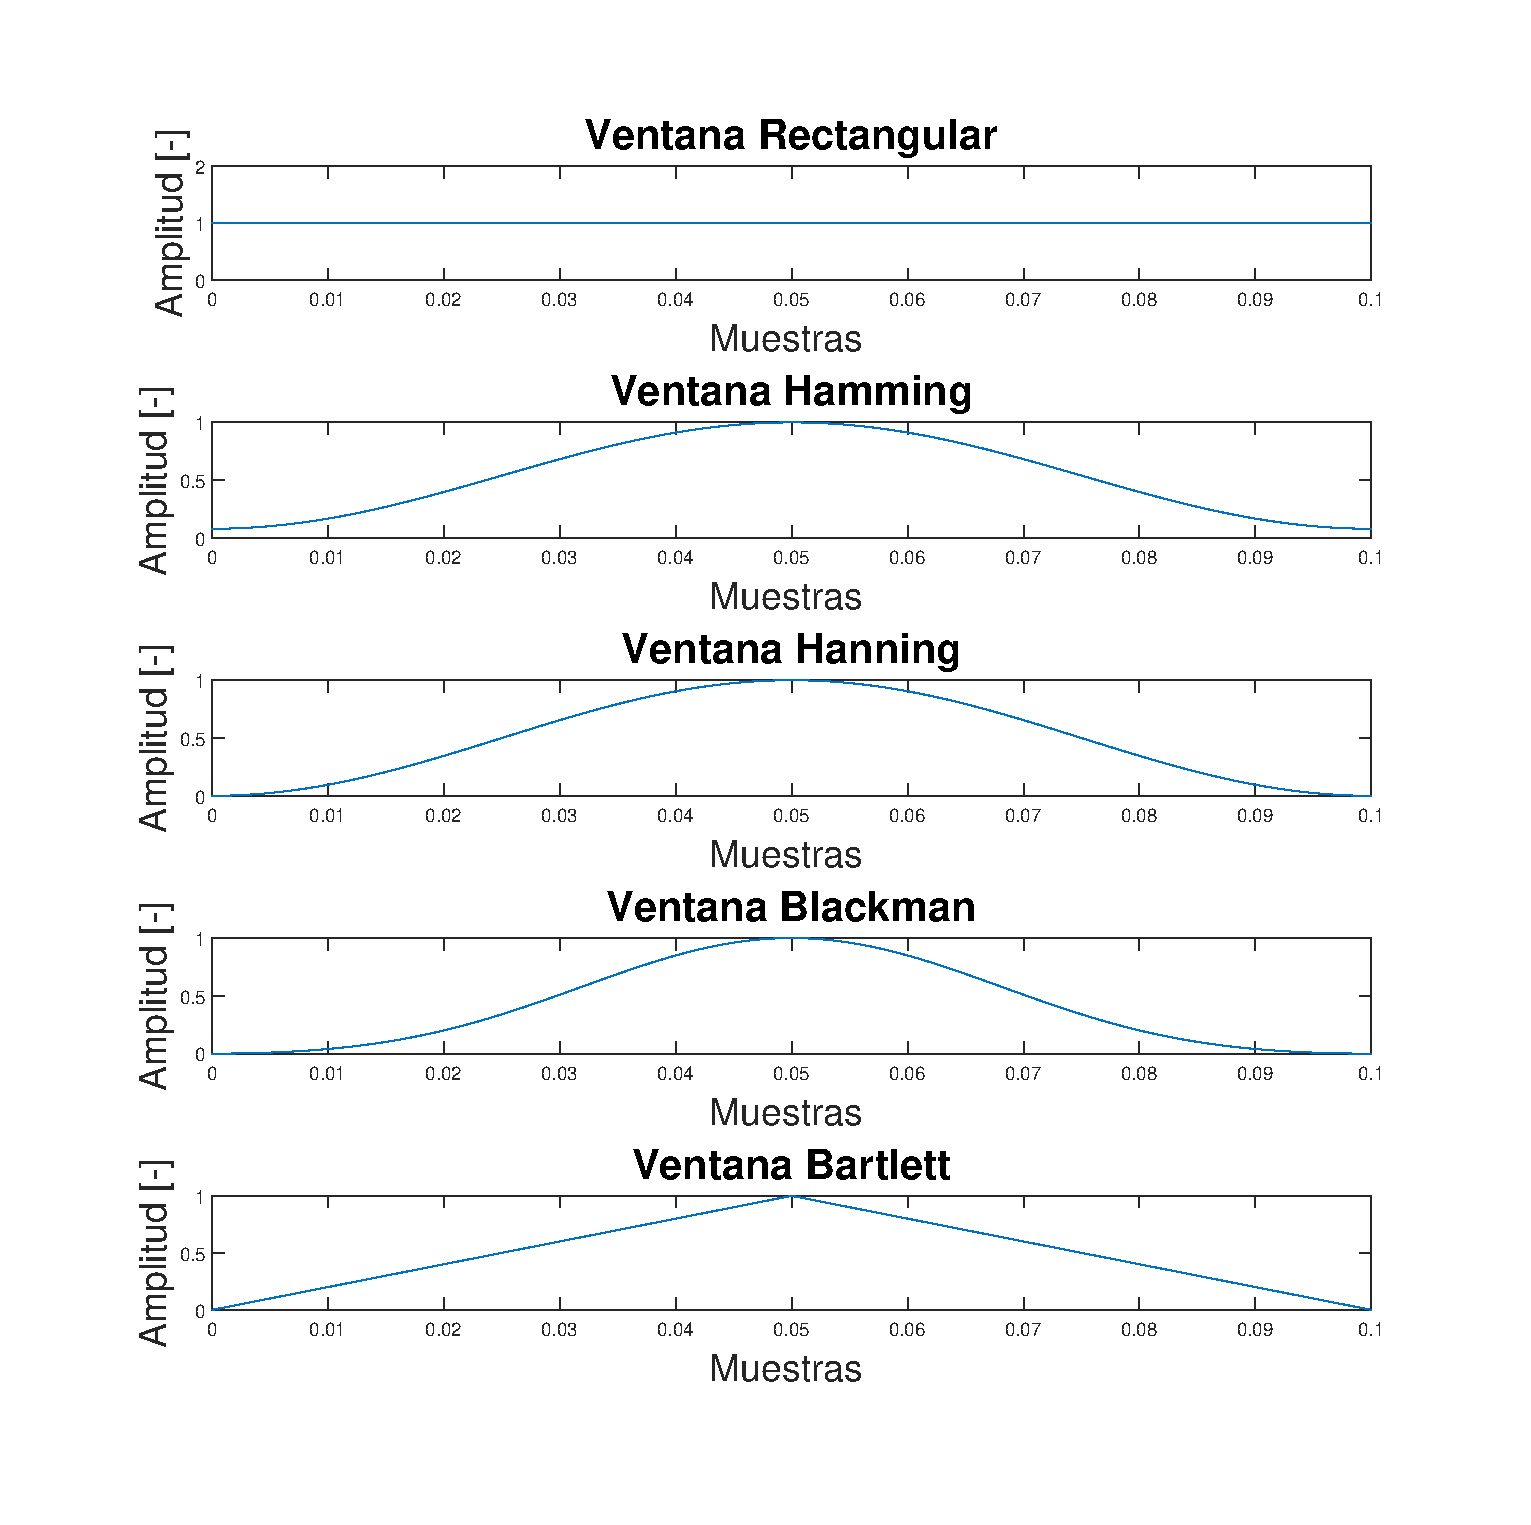
\includegraphics[scale = 0.5]{Figuras/p2_2-Ventanas-tiempo.eps}
    \caption{Ventanas rectangular, hamming, hanning, blackman, y bartlett en el tiempo.}
    \label{ventanas_tiempo}
\end{figure}


En la figura \ref{ventanas-magnitud} se puede ver cual es el comportamiento en  frecuencia de cada uno de los tipos de ventanas utilizadas.

\begin{figure}[H]
    \centering
    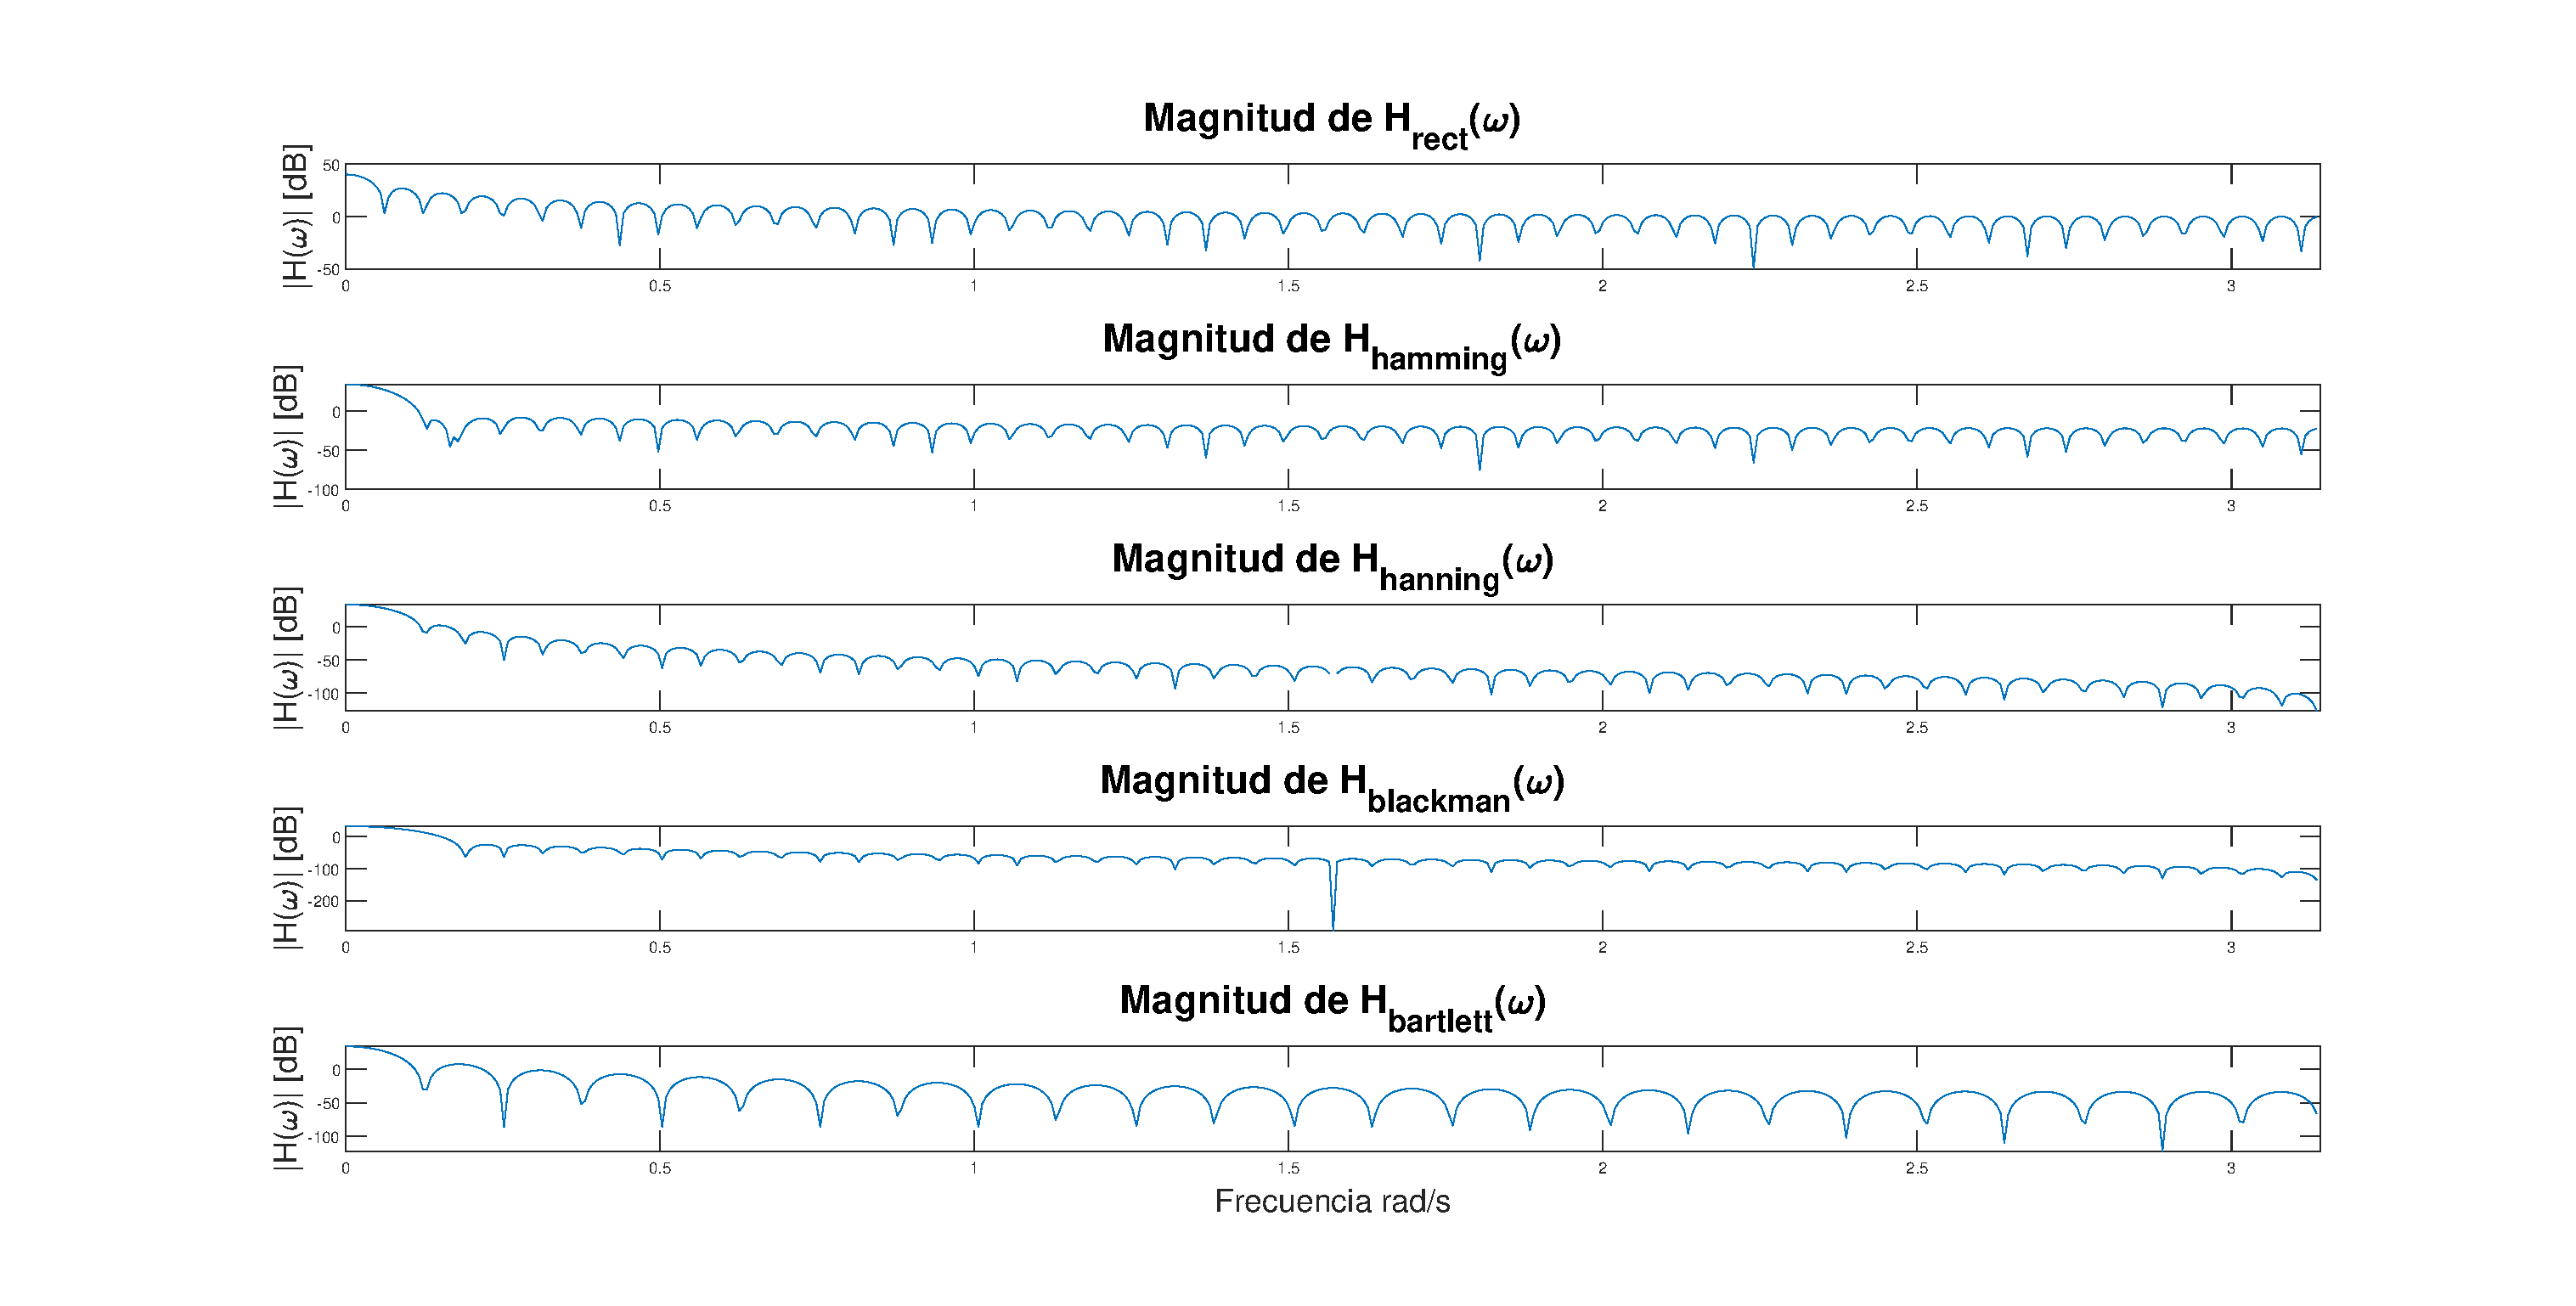
\includegraphics[scale = 0.3]{Figuras/p2_2-Ventanas-frecuencia.eps}
    \caption{Magnitud de ventanas rectangular, hamming, hanning, blackman, y bartlett en frecuencia.}
    \label{ventanas-magnitud}
\end{figure}


En la figura \ref{vent-mag-fase} se observa el comportamiento de las ventanas en frecuencia con énfasis en las frecuencias cercanas a cero, donde se pueden observar el ancho del \textit{mainlobe} de la ventana, además de la fase correspondiente a la ventana.

\begin{figure}[H]
    \centering
    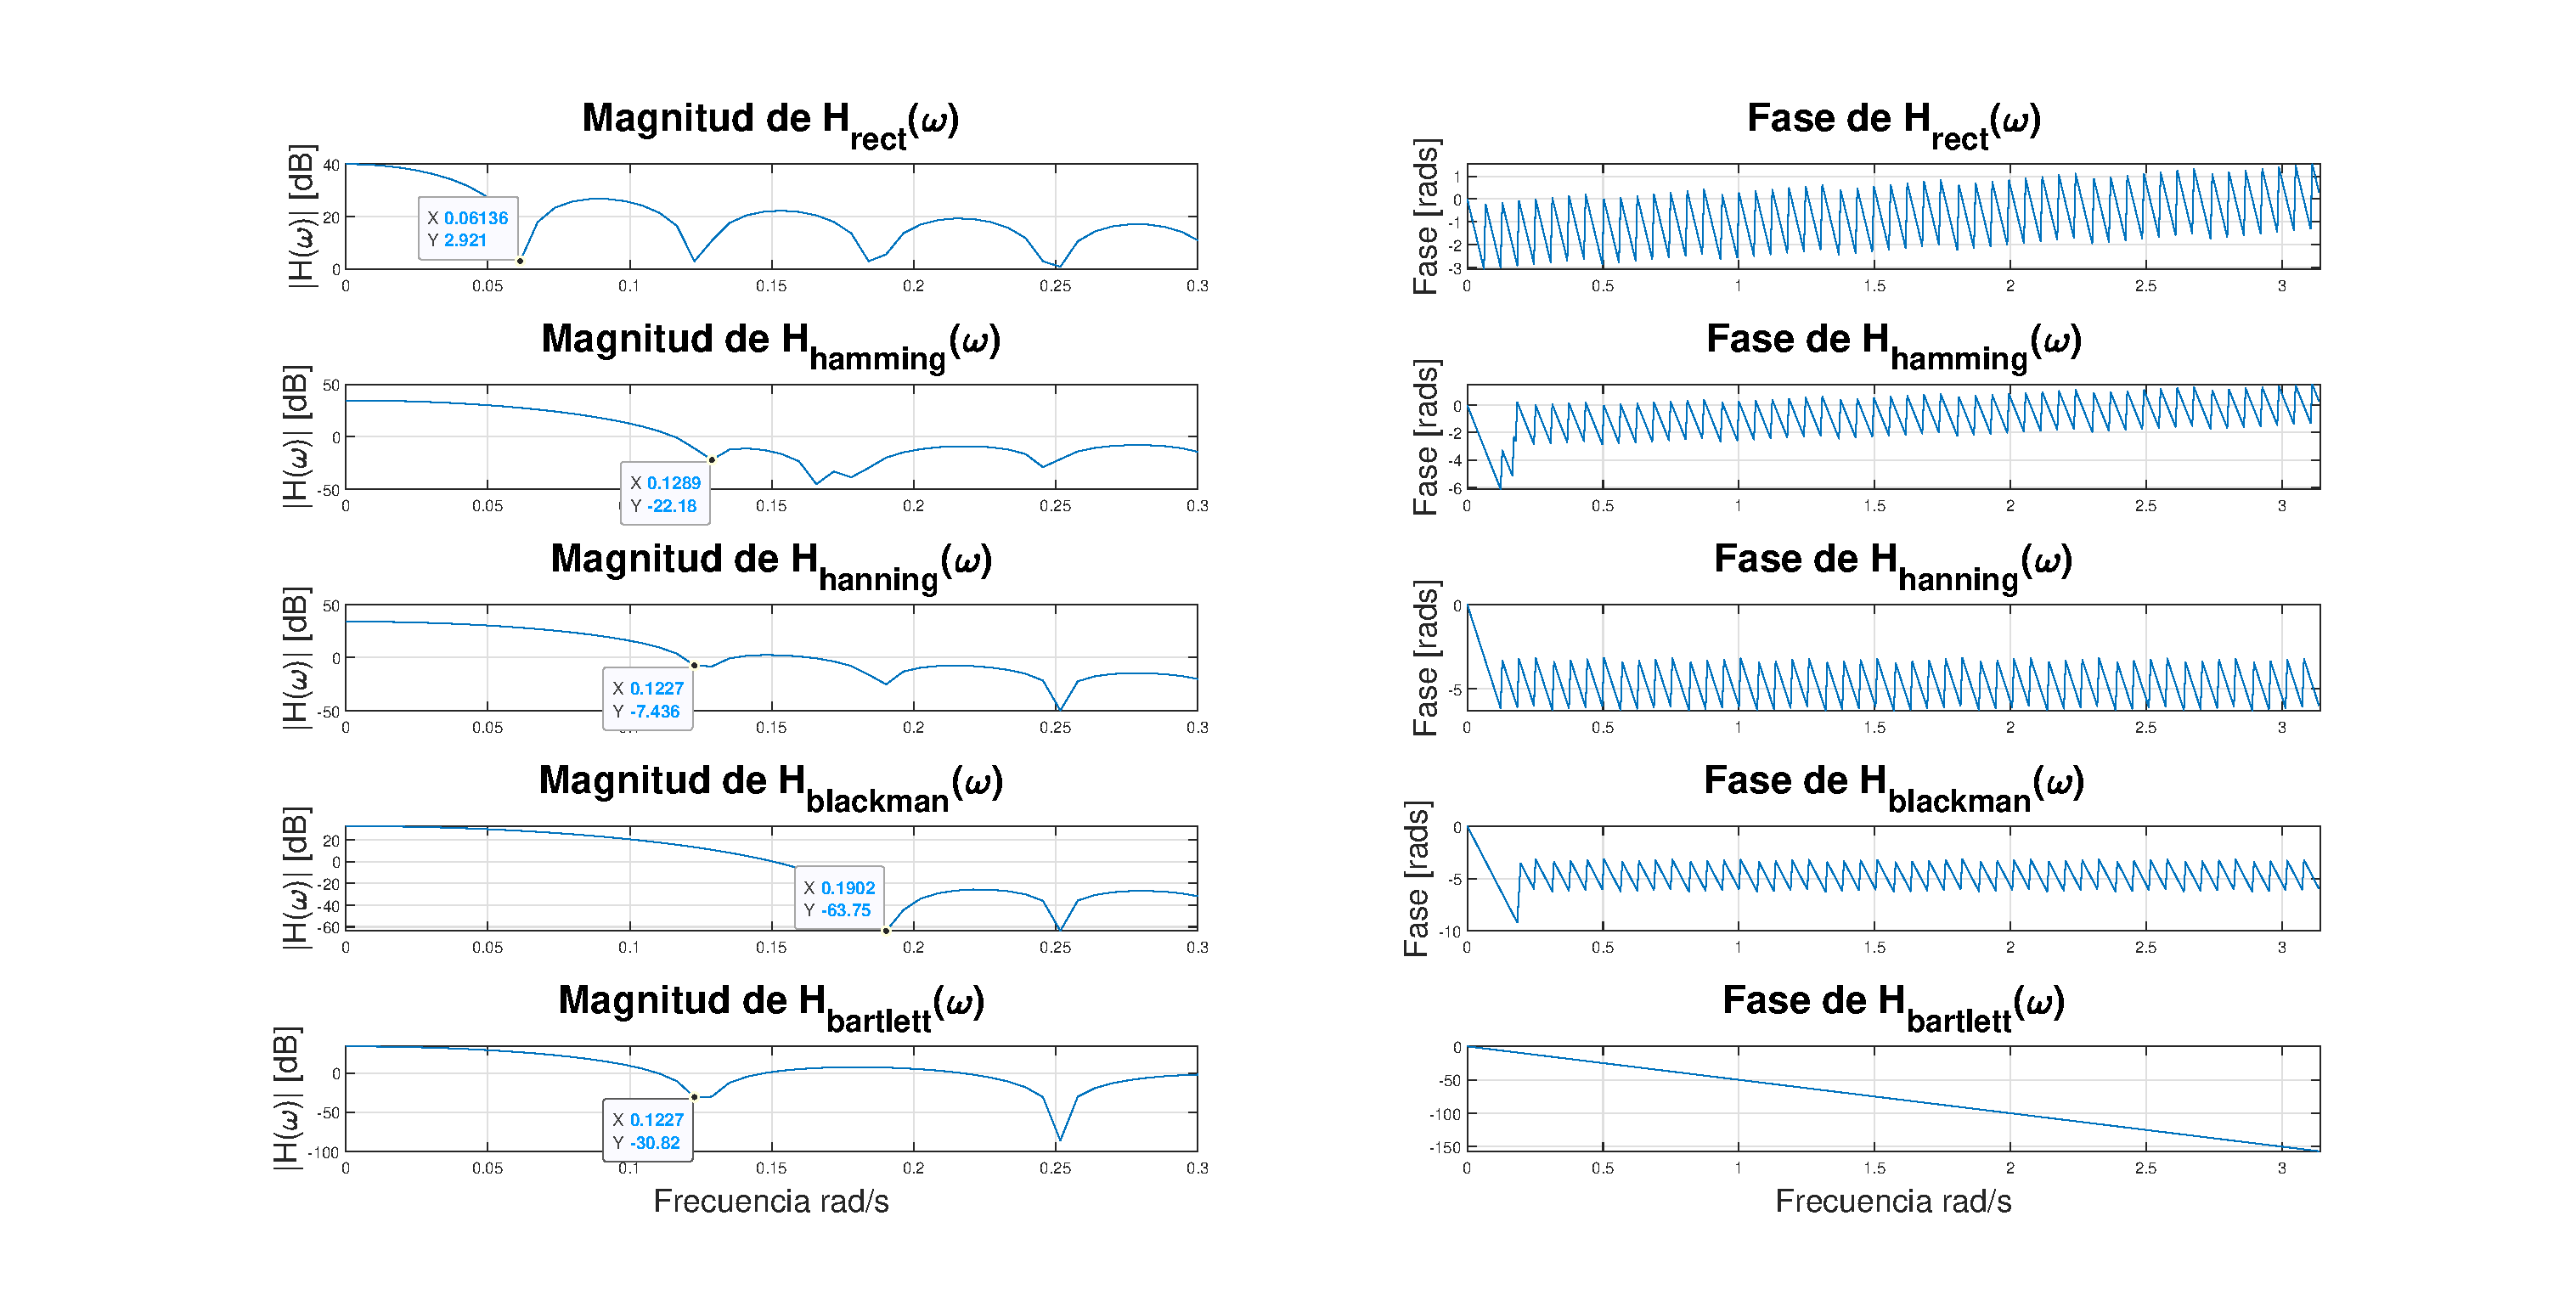
\includegraphics[scale = 0.3]{Figuras/p2_2-Magnitud-Fase.eps}
    \caption{Magnitud  y fase de ventanas rectangular, hamming, hanning, blackman, y bartlett en frecuencia. }
    \label{vent-mag-fase}
\end{figure}

En la figura \ref{lobulos}, se pueden ver los valores máximos que toman el \textit{mainlobe} y el \textit{sidelobe} para cada tipo de ventana, valores se resumen en el cuadro \ref{resumen_ventanas} junto al ancho del \textit{mainlobe}  de cada ventana obtenido anteriormente


\begin{figure}[H]
    \centering
    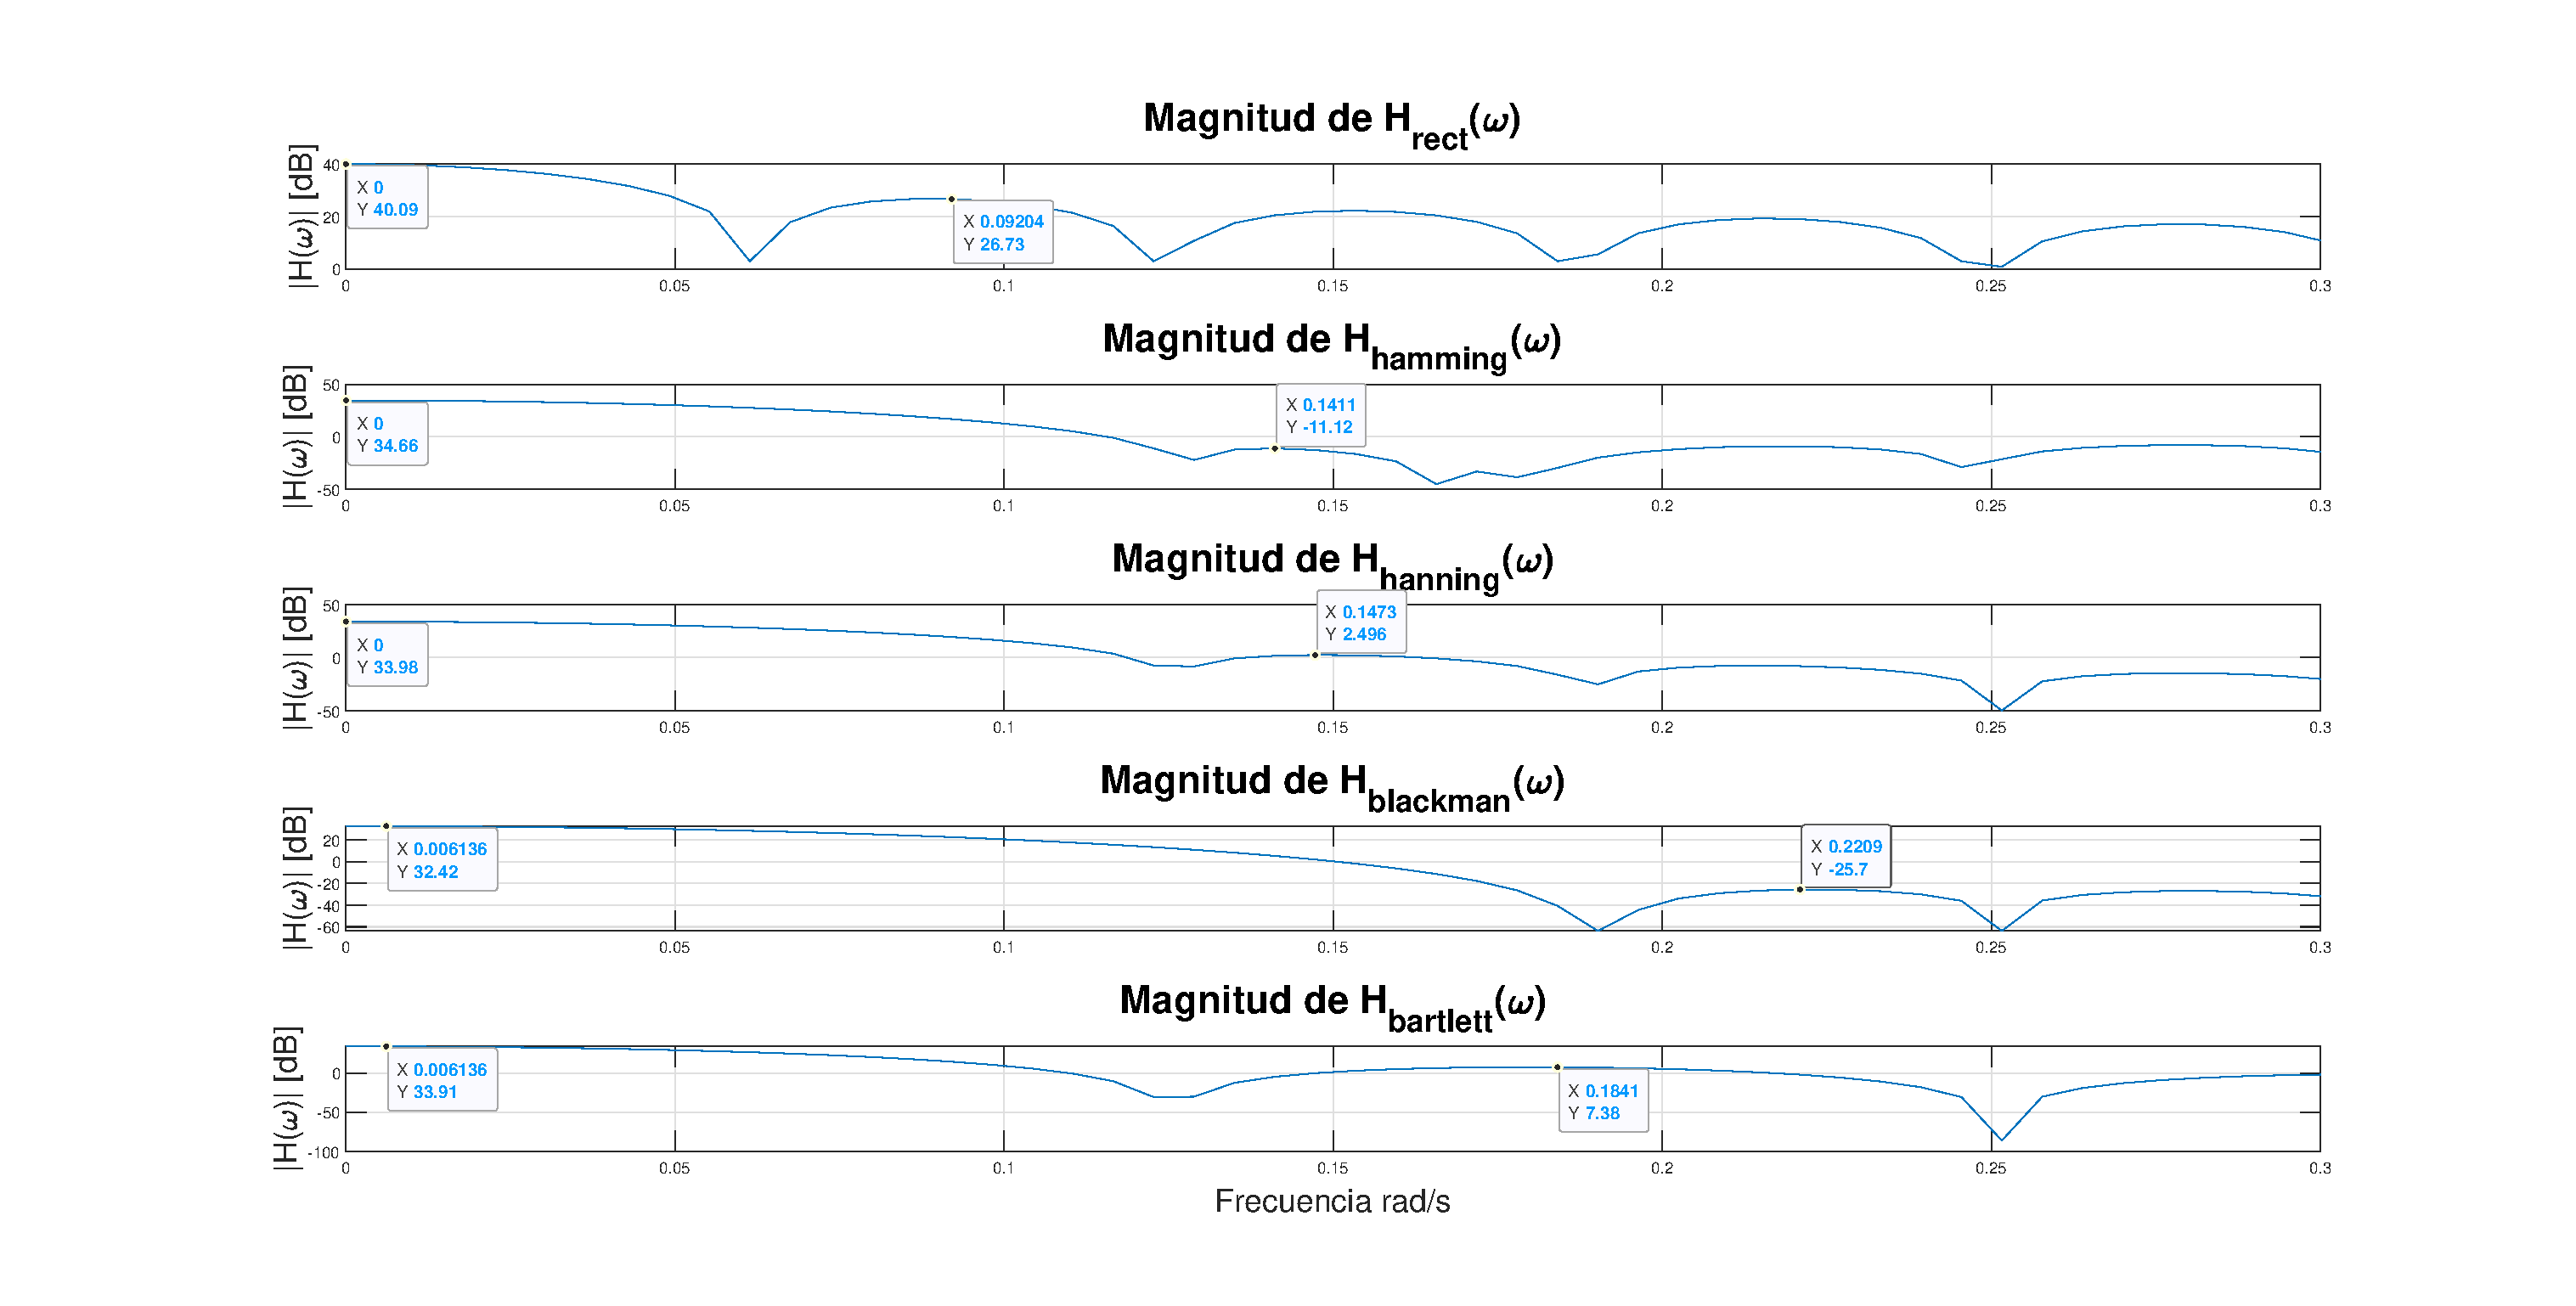
\includegraphics[scale = 0.3]{Figuras/p2_2-Lobulos.eps}
    \caption{Magnitud de ventanas rectangular, hamming, hanning, blackman, y bartlett en frecuencia identificando la amplitud del \textit{mainlobe} y el \textit{sidelobe}.}
    \label{lobulos}
\end{figure}


 Como todas las magnitudes se encuentran medidas en $db$ para encontrar la amplitud relativa de el \textit{sidelobe} basta con hacer la resta de la amplitud de este último con la amplitud del \textit{mainlobe}
 
 \begin{table}[H]
        \centering
        \begin{tabular}{|c|c|c|c|c|c|c|}
        \hline
         Ventana   & Ancho mainlobe & Max mainlobe & Max sidelobe & Amplitud relativa sidelobe\\
         \hline
         Rectangular  & 0.06136	 &  40.09 &	26.73	& -13.36 \\
         \hline
         Hamming  & 0.1289 &	34.66	& -11.12 &	-45.78	 \\
         \hline
         Hanning & 0.1227	& 33.98 &	2.496 &	 -31.484  \\
         \hline
        
         Blackman  & 0.1902 &	32.42	& -25.7 &	-58.12\\
         \hline
        
        Bartlett  & 0.1227 &	33.91	& 7.38 &	-26.53	\\
         \hline

        \end{tabular}
        \caption{Ancho \textit{mainlobe} y relación entre amplitud de \textit{mainlobe} y  \textit{sidelobe} en $db$}
        \label{resumen_ventanas}
    \end{table}

     De la tabla anterior se observa que la ventana rectangular es la ventana que tiene un sidelobe con mayor amplitud relativa, es decir, en cuanto a eficacia del filtro este es el menos óptimo.  Los filtros que poseen una mayor atenuación para las frecuencias fuera de su frecuencia de corte son los implementados con ventanas \textit{Hamming} y \textit{Blackman}, pero cabe mencionar que esta última compromete el ancho del lóbulo principal para lograr la atenuación que provee, esto podría generar conflictos dependiendo de lo que se busca en la implementación del filtro.  Los filtros con ventanas de tipo \textit{Hanning} y \textit{Bartlett} tienen un desempeño intermedio entre  el desempeño de ventana rectangular y el desempeño con ventanas \textit{Hamming} y/o \textit{Blackman}.

\end{enumerate}